\documentclass[sigconf, anonymous]{acmart}

%!TEX root = ../main.tex
\newcommand{\eat}[1]{}
\usepackage{latexsym}
\usepackage{amsfonts}
\usepackage{amsmath}
%\usepackage{amssymb}
\usepackage{color}
\usepackage{colortbl}
\usepackage{epsfig}
\usepackage{xspace}
\usepackage{graphicx}
\usepackage{subfigure}
\usepackage{pifont}
\usepackage{bm}
\usepackage{bbding}

%\usepackage{algorithmicx}
\usepackage{xparse}

\usepackage[lined,boxed,vlined,ruled,linesnumbered]{algorithm2e}
\usepackage{algorithmicx}
\usepackage{paralist}
\usepackage{enumerate}
\usepackage{ifthen}
\usepackage{ulem}
\usepackage{makecell}

%response command
\newcommand{\stitle}[1]{\vspace{1.2ex}\noindent{\bf #1}}
\newcommand{\etitle}[1]{\vspace{0.8ex}\noindent{\underline{\textit{#1}}}}
\newcommand{\ititle}[1]{\vspace{1ex}\noindent\textbf{\textit{#1}}}
\newcommand{\overwrite}[1]{\textcolor{blue}{#1}}
\newcommand{\bfit}[1]{\textbf{\textit{#1}}}
\newcommand{\re}[1]{\noindent{\textbf{\textit{#1}}}}
%%%%%%%%%%%%%%%%%%%%%%%%%%%%%%%%%%%%%
%% DO NOT DELETE!!
%%%%%%%%%%%%%%%%%%%%%%%%%%%%%%%%%%%%%
%\usepackage{tikz}
%\usetikzlibrary{trees}

\usepackage{epsfig}
\usepackage{multirow}
\usepackage{url}

\usepackage[color,matrix,arrow,all]{xy}
%\usepackage[all,cmtip]{xy}

\usepackage{tikz}
\usetikzlibrary{shapes,snakes}
\usetikzlibrary{calc}

\newtheorem{example}{Example}
\newtheorem{theorem}{Theorem}

\newcommand{\add}[1]{\textcolor{blue}{#1}}
\newcommand{\lgl}[1]{\textcolor{blue}{#1}}
\NewDocumentCommand{\cc}{ mO{} }{\textcolor{red}{\textsuperscript{\textit{CC}}\textsf{\textbf{\small[#1]}}}}

\newcommand{\addnew}[1]{\textcolor{red}{#1}}


\NewDocumentCommand{\wjy}{ mO{} }{\textcolor{violet}{\textsuperscript{\textit{WJY}}\textsf{\textbf{\small[#1]}}}}

\NewDocumentCommand{\nan}{ mO{} }{\textcolor{blue}{\textsuperscript{\textit{nan}}\textsf{\textbf{\small[#1]}}}}

\sloppy
\newcommand{\rtable}[1]{\ensuremath{\mathsf{#1}}}
\newcommand{\ratt}[1]{\ensuremath{\mathit{#1}}}
\newcommand{\stt}[1]{\texttt{\small{#1}}}
\newcommand{\at}[1]{\protect\ensuremath{\mathsf{#1}}\xspace}
\newcommand{\myhrule}{\rule[.5pt]{\hsize}{.5pt}}
\newcommand{\oneurl}[1]{\texttt{#1}}
\newcommand{\tabstrut}{\rule{0pt}{4pt}\vspace{-0.1in}}
\newcommand{\stab}{\vspace{1.2ex}\noindent}
\newcommand{\sstab}{\rule{0pt}{8pt}\\[-2.2ex]}
\newcommand{\vs}{\vspace{1ex}}
\newcommand{\exa}[2]{{\tt\begin{tabbing}\hspace{#1}\=\+\kill #2\end{tabbing}}}
\newcommand{\ra}{\rightarrow}
\newcommand{\match}{\rightleftharpoons}


\newcommand{\sys}{\texttt{TD-Bench}\xspace}

%%%%%%%%%%%%%%%%%%%%%%%%%%%%%%%%%%%%%%%%
%%%%%%%%%%%%%%%%%%%%%%%%%%%%%%%%%%%%%%%%
\newcommand{\qtable}{T_q}
\newcommand{\qcolumn}{C_q}
\newcommand{\tcolumn}{C_t}
\newcommand{\ttable}{T_t}
\newcommand{\lake}{\mathcal{T}}


\newcommand{\jqtable}{T^J_q}
\newcommand{\uqtable}{T^U_q}
\newcommand{\jqcolumn}{C^J_q}
\newcommand{\jtcolumn}{C^J_t}




\newcommand{\querycolumnnum}{\mathcal{P}}
\newcommand{\dlllneighbornnum}{\mathcal{D}}
\newcommand{\inforneighbornnum}{\mathcal{I}}
\newcommand{\averagetargettuplenum}{\overline{\mathcal{O}}}
\newcommand{\tuplenum}{\mathcal{X}}
\newcommand{\tablenum}{\mid \mathcal{T} \mid}
\newcommand{\columnnum}{\mathcal{N}}
\newcommand{\cellnum}{\mathcal{M}}
\newcommand{\rawtokennum}{\mathcal{R}}
\newcommand{\cellvaluenum}{\mathcal{K}}
\newcommand{\positinglistlen}{\mathcal{L}}
\newcommand{\minhashlen}{\mathcal{H}}
\newcommand{\lshpart}{\mathcal{B}}
\newcommand{\querycellvalue}{\mathcal{A}}

\newcommand{\josie}{Joise\xspace}
\newcommand{\lsh}{LSH Ensemble\xspace}
\newcommand{\pex}{Pexeso\xspace}
\newcommand{\deepjoin}{DeepJoin\xspace}
\newcommand{\tus}{TUS\xspace}
\newcommand{\dlll}{D3L\xspace}
\newcommand{\starmie}{Starmie\xspace}
\newcommand{\santos}{Santos\xspace}
\newcommand{\frt}{Frt12\xspace}
\newcommand{\infogather}{InfoGather\xspace}
\newcommand{\aurum}{Aurum\xspace}

%%%%%%%%%%%%%%%%%%%%%%%%%%%%%%%%%%%%%%%%
%%%%%%%%%%%%%%%%%%%%%%%%%%%%%%%%%%%%%%%%

\newcommand{\la}{\leftarrow}
\newcommand{\bi}{\begin{itemize}}
	\newcommand{\ei}{\end{itemize}}
\newcommand{\mat}[2]{{\begin{tabbing}\hspace{#1}\=\+\kill #2\end{tabbing}}}
\newcommand{\be}{\begin{enumerate}}
	\newcommand{\ee}{\end{enumerate}}
\newcommand{\beqn}{\begin{eqnarray*}}
	\newcommand{\eeqn}{\end{eqnarray*}}

\newcommand{\ie}{$i.e.$,\xspace}
\newcommand{\eg}{$e.g.$,\xspace}
\newcommand{\wrt}{w.r.t.\xspace}
\newcommand{\aka}{a.k.a.\xspace}
\newcommand{\kwlog}{\emph{w.l.o.g.}\xspace}

\newcommand{\eop}{\hspace*{\fill}\mbox{$\Box$}\vspace{1ex}}     % End of proof

\makeatletter
\newcommand\figcaption{\def\@captype{figure}\caption}
\newcommand\tabcaption{\def\@captype{table}\caption}
\makeatother

\newcommand{\reminder}[1]{ {\mbox{$<==$}} [[[ \bluefont{ \bf #1 } ]]] {\mbox{$==>$}}}

\definecolor{shadecolor}{RGB}{220,220,220}
\newcommand{\mybox}[1]{\vspace{1.5ex}\par\noindent\colorbox{shadecolor}
	{\parbox{\dimexpr\columnwidth-2\fboxsep\relax}{#1}}\vspace{1ex}}


\tikzstyle{mybox} = [draw=black, fill=black!5, thick,
rectangle, rounded corners, inner sep=0pt, inner ysep=2pt]
\tikzstyle{fancytitle} =[fill=black, text=white]











%\settopmatter{printacmref = false}

\renewcommand\footnotetextcopyrightpermission[1]{}

%% \BibTeX command to typeset BibTeX logo in the docs
\AtBeginDocument{%
	\providecommand\BibTeX{{%
			Bib\TeX}}}
		 
%% These commands are for a PROCEEDINGS abstract or paper.
\acmConference[SIGMOD' 24]{Make sure to enter the correct
	conference title from your rights confirmation emai}{June 11--16,
	2024}{Santiago, Chile}

\begin{document}
\title{Table Discovery Benchmark}


\renewcommand{\shortauthors}{Trovato et al.}

\begin{abstract}
Recently, table discovery has attracted much attention because 
\end{abstract}

\maketitle

%!TEX root = ../main.tex

\section{Introduction}
 
Nowadays, the number of open datasets from multiple sources ($e.g.,$ governments and companies) keeps growing, which provides large potential opportunity for intelligent data analysis. However, these datasets are always stored in the data lake that are not well-organized like storing in a database with well-defined schemes and indexes. Hence, it is challenging to efficiently and effectively find user-required data considering the data lake scale and the semantics of user requirements.  
To exploit the enormous value in the data lake, researchers from both industry and academia have implemented a number of data discovery engines~\cite{} that retrieve relevant user-specified tables. 


%given a query table, they search relevant tables from the data lake, so as to benefit the downstream applications, such as augmenting more data instances~\cite{} or  improving the machine learning model performance~\cite{}. 

\begin{table*}[t]
	\centering
	\caption{Benchmark Comparison.}
	\begin{tabular}{|c|c|c|c|c|c|c|}
		\hline
		\centering
		Benchmarks & Type & $\#$-Query tables & $\#$-Lake tables & $\#$-Total columns & Size (GB) &  API \\
		\hline  
		TUS Small~\cite{TUS}& Union  & 200 & 1,530 & 14,810 & 1 & \XSolidBrush \\
		\hline
		TUS Large~\cite{TUS}& Union  & 1,000 & 5,043 & 54,923 & 1.5 & \XSolidBrush \\
		\hline
		Santos Small~\cite{Santos}& Union  & 50 & 550 & 6,322 & 0.45 & \XSolidBrush \\
		\hline
		Santos Large~\cite{Santos}& Union  & 80 & 11,090 & 123,477 & 11 & \XSolidBrush  \\
		\hline
		Josie~\cite{Josie}& Join  & XX & XX  & XX  & XX &  \XSolidBrush \\
		\hline
		Valentine~\cite{valentine}& XX  & XX & XX  & XX  & XX &  \XSolidBrush \\
		\hline
		LakeBench~\cite{arxiv}& Union & XX & XX  & XX  & XX &  \XSolidBrush \\
		\hline
		\rowcolor{gray!40}
		OpenData Small& Join \& Union  & XX & XX  & XX  & XX & \Checkmark  \\
		\hline
		\rowcolor{gray!40}
		OpenData Large& Join \& Union  & XX & XX  & XX  & XX & \Checkmark  \\
		\hline
		\rowcolor{gray!40}
		WebTable Small& Join \& Union  & XX & XX  & XX  & XX & \Checkmark\\
		\hline
		\rowcolor{gray!40}
		WebTable Large& Join \& Union  & XX & XX  & XX  & XX &\Checkmark \\
		\hline
	\end{tabular}
	\label{Table:benchmarks}

\end{table*}

In general, discovering related tables from data lakes can be generally categorized into several sub-tasks, namely keyword-based search, joinable table search and unionable table search.
The first category~\cite{} issues keywords as queries, based on which relevant tables are retrieved. 
We focus on the latter two categories that issue a table as the query, which have recently attracted much attention because they are widely-used for augmenting more data instances~\cite{} or features~\cite{}, so as to  benefit the downstream applications like machine learning based data analysis.
%


To be specific, given a query table with a user-specified column, joinable table search finds the target tables that can be joined with the column.

\begin{example}
	As shown in Figure~\ref{fig:example}(a), given the query table ($T_1$) and a specified column \texttt{Corporation},  
	we can observe that Table $T_2$ in the data lake is joinable, \ie the first attribute of $T_2$ can be joined with the specified column mainly because i). the column names are  matching  and 
	ii). there exist a number of semantically overlapping cell values (\eg Apple and Apple Inc.). 
	%
	The joined table can be taken as feature augmentation to improve model performance when  the \texttt{Price} is treated as the predicted column. 
	%
	In addition, although the first attribute of $T_3$ has a semantically similar column name and contents  with the specified column, it is not joinable because there is no overlapping values.
\end{example}

 For unionable table search, given a query table, it aims to find target tables that are unionable with the query from the data lake.                  
 
 \begin{example}
 	As shown in Table~\ref{fig:example}(b), given a query table ($T_4$)  for searching unionable tables, we find that  $T_5$ can be unioned with $T_4$ because they are all about the information of movies and  two pairs of attributes are highly correlated ($T_4$.\texttt{Name} $v.s.$ $T_5$.\texttt{Movie} and $T_4$.\texttt{Rating} $v.s.$ $T_5$.\texttt{Score}). 
 	However, when it comes to $T_6$, we can observe that there exist three attributes ($T_6$.\texttt{City}, $T_6$.\texttt{Date} and $T_6$.\texttt{Rating}) that can be respectively aligned with attributes ($T_4$.\texttt{Venue}, $T_4$.\texttt{Date} and $T_4$.\texttt{Rating}) of $T_4$,  $T_6$ is not unionable with the query $T_4$ because the two tables are totally not semantically relevant ($T_4$ is about movies while $T_6$ is about restaurants).
 \end{example}



\begin{figure*}[h]
	\centering
	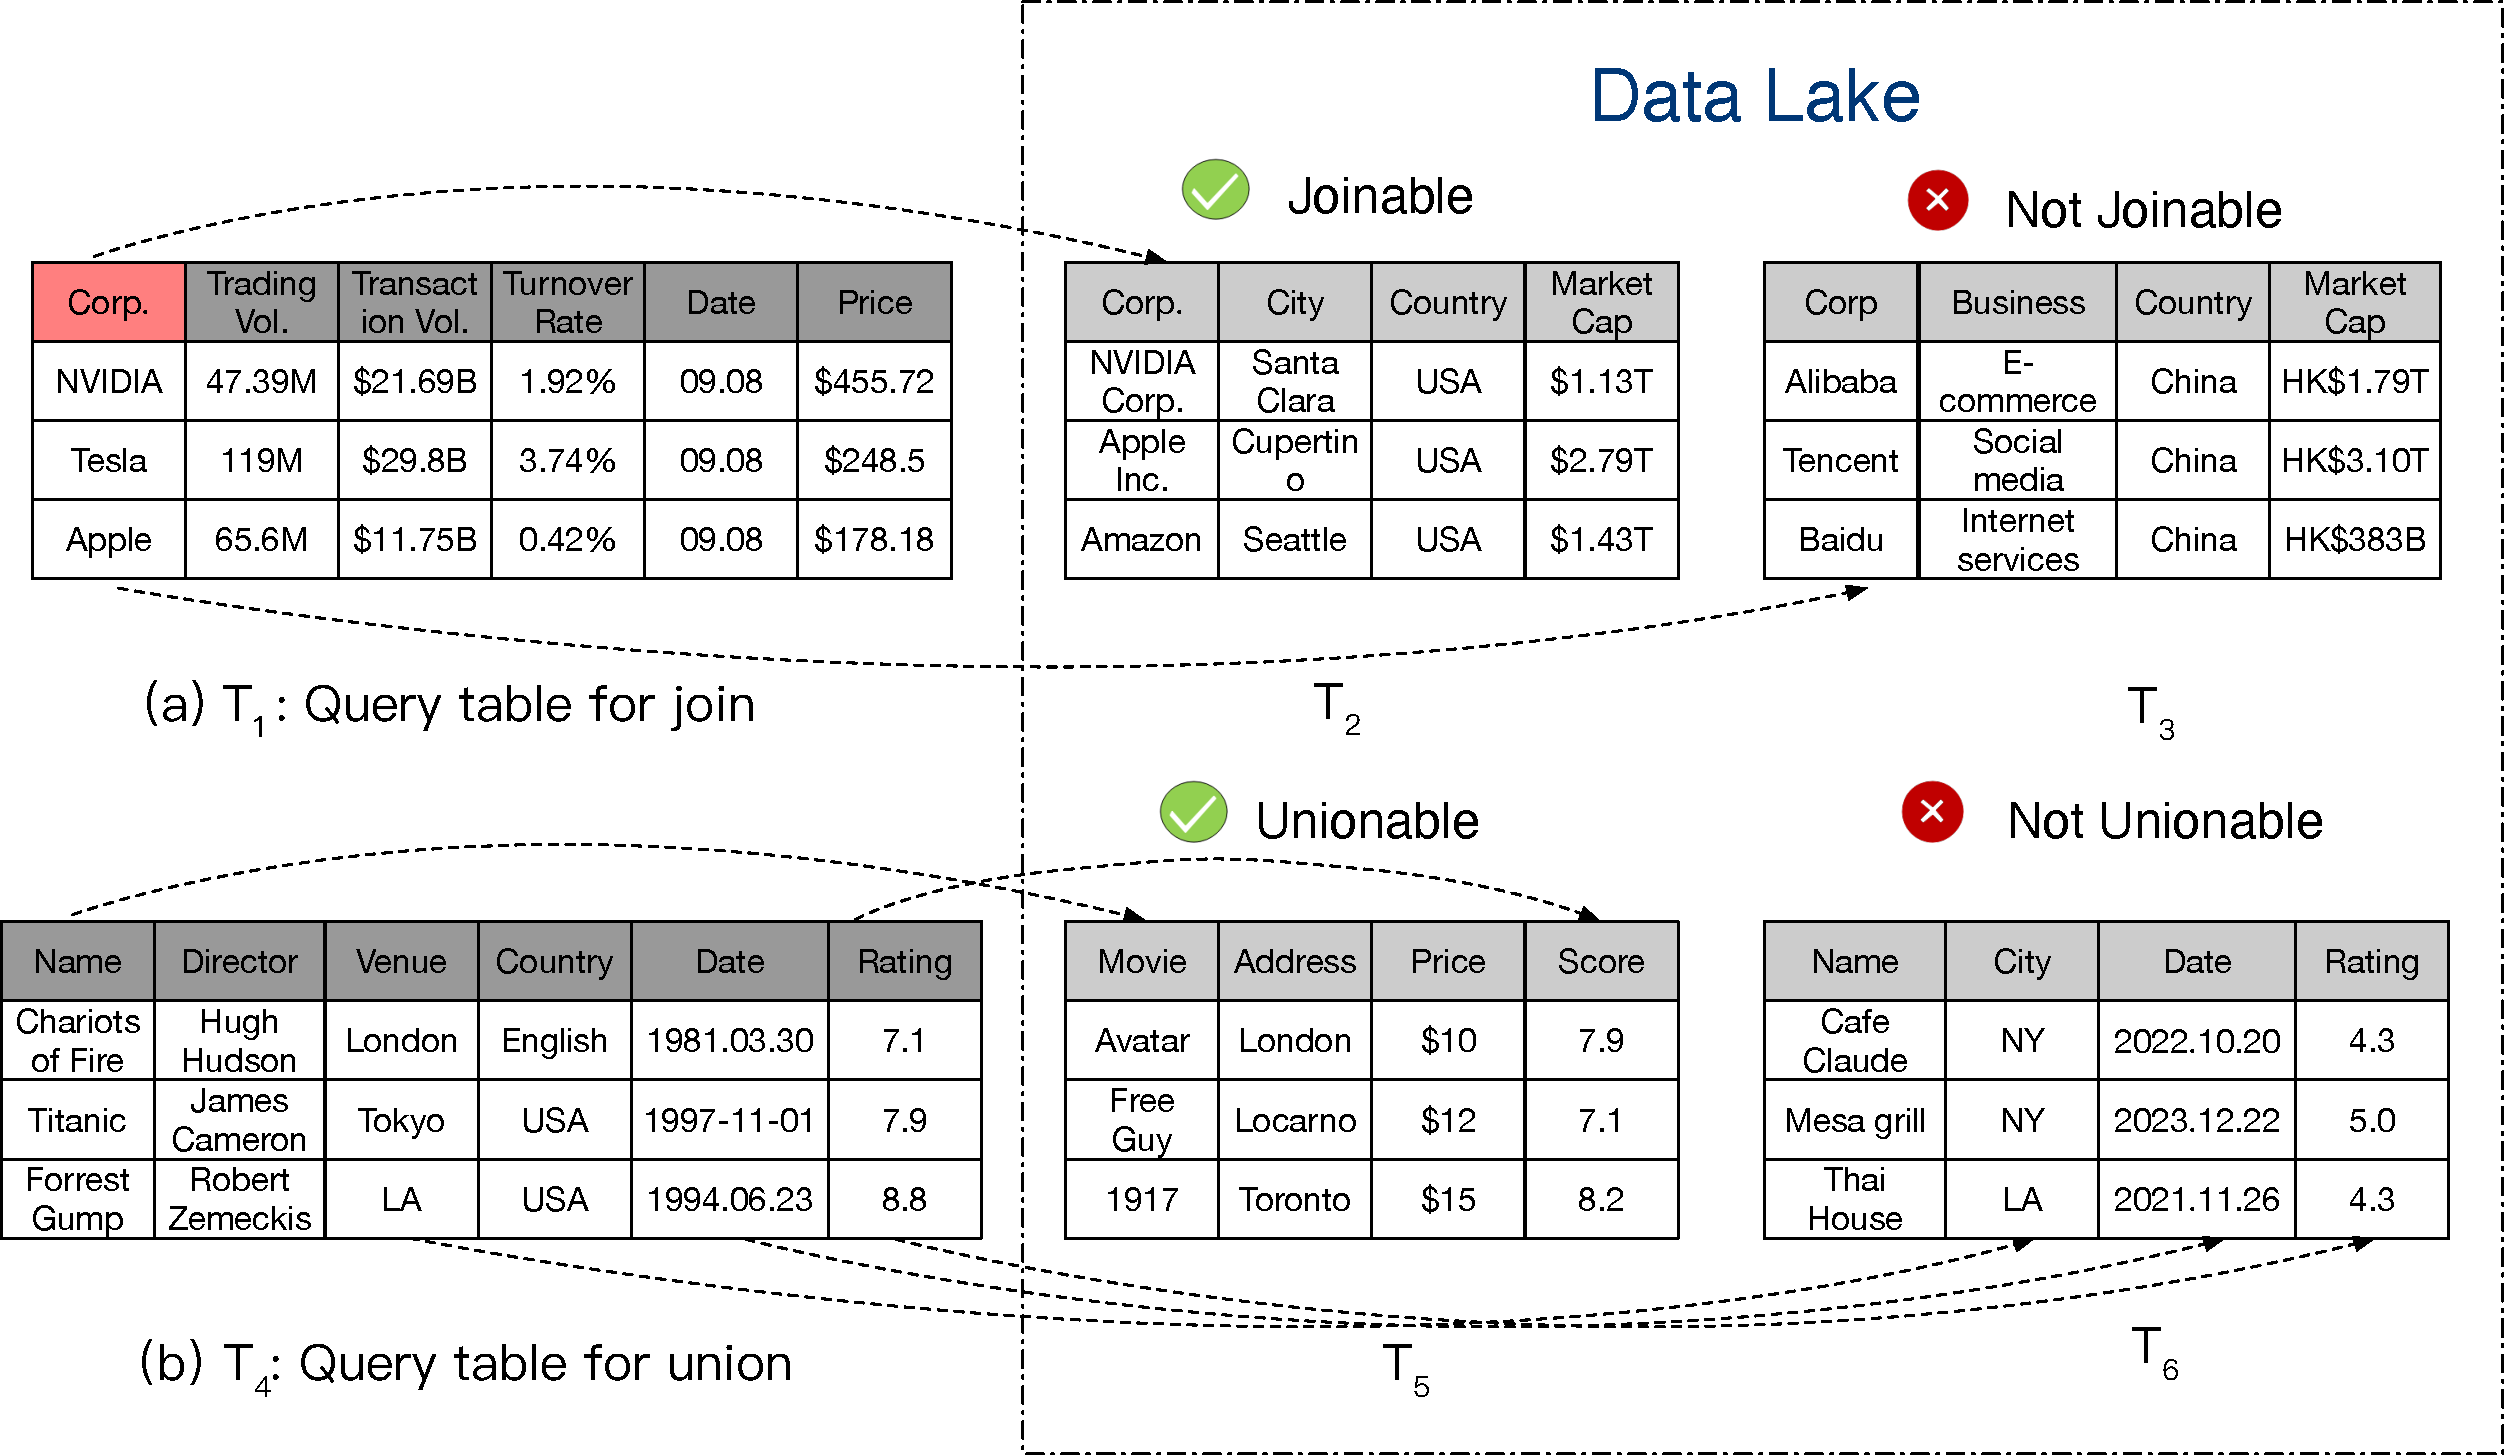
\includegraphics[width=0.8\linewidth]{fig/example.pdf}
	\caption{Table Discovery in Data Lake.}
	\label{fig:example}
\end{figure*}


From the above examples, we can see that table discovery from the data lake is a non-trivial task we should consider (1) the semantic schema similarity of columns, (2) the (semantic) overlappings between columns as well as the (3) contextual information of all columns in a table.
What's more, as the data lake is always large-scale, the efficiency is also a challenging problem. Despite its importance and hardness, existing approaches have still not been evaluated  sufficiently due to the lack of a comprehensive benchmark.  In retrospect, benchmarks have played a significant role
in spawning the boom in different research communities, such as
TPC benchmarks~\cc{\cite{}} for the database community, ImageNet~\cc{\cite{}} for computer vision tasks, and GLUE~\cc{\cite{}} for natural language processing tasks.



\nan{
\bi
	\item Intro
	\be
		\item Sec~1 Add a table or several tables to compare the number of tables/queries supported by your benchmark and others'. 
		\item Easy-to-use APIs: maybe you can give examples for designed unified APIs, saying learned from Hugging Face. They can easily compare different methods. 
		\item Leaderboard.
	\ee
	\item Sec~3 Benchmark design: align with the revised intro
	\item Sec~4 Statistics of datasets, Sec~5 Statistics of queries -- they can be merged if each section is short
	\item Annotation process
	\item API design can be pushed before ``Analyzing benchmark results''
\ei
}




\noindent \textbf{Existing Benchmarks.}  
TUS~\cite{TUS} first builds a benchmark for table union search, which contains around 5,000 tables (from OpenData) in the data lake, among which 1,000 queries are selected as query tables with ground truth. 
Santos~\cite{Santos} improves the TUS benchmark by additionally labeling column-to-column relations to consider more semantics, but it is just for table union search with around 10,100 data lake tables and 80 query tables.
Josie~\cite{Josie} is a join search benchmark that uses two data lakes. One is the same with TUS, and the other is sampled from the Web Table, with 1,000 query columns respectively. 
Valentine~\cite{valentine} evaluates multiple schema matching techniques to solve table discovery tasks, using several hundreds of tables to match pairs of tables. A recent Arxiv work~\cite{arxiv} focuses on evaluating table pretraining methods for table discovery tasks, with the goal of improve downstream machine learning tasks. 

\noindent \textbf{Challenges.} Overall, benchmarking table discovery in data lake faces several major challenges.

\noindent (1) [\textit{Data/Query Coverage}] The effectiveness and efficiency of table discovery largely rely on the characteristics of datasets, like the data lake scale, average column/instance number per table etc. Also, different query  characteristics also lead to different performance, such as query column/table size,  query column type,  result size etc. 

\noindent (2) [\textit{Ground Truth Labeling}] 
 Most existing benchmarks have limited number of queries,  mainly because it is rather expensive to label the ground truth (tables  that can join/union with query in data lake) for each query table. Hence, it is non-trivial to create sufficient queries with ground truth to evaluate different table search approaches.

\noindent (3) [\textit{Solution Coverage}] 
Recently, several unionable/joinable table search methods have been proposed, but there lacks of a thorough comparison over these methods.

\noindent (4) [\textit{User-friendly Interface for Benchmark Usage}] Existing benchmarks just provide datasets, queries and ground truth, which is not very user-friendly if a user wants to
run different algorithms over these benchmarks.


To address the above challenges, in this paper, we create a comprehensive benchmark \sys for table search in data lake.

 First, we collect 3 TB tables from different sources, including OpenData~\cite{} and  WebTable~\cite{}, based on which we evaluate different the table union/join search approaches. These datasets have diverse characteristics. WebTable has a large number of tables (XXX) but each has a small size. In contrast, each table in OpenData is quite large (XXX), but the number is smaller than that of WebTable. 
 
 
Second, we create sufficient and diverse queries using two approaches. 
One is to split big tables in data lake into small ones, put these small tables into the data lake and they can be naturally joined or unioned. Hence, when these small tables serve as queries, the ground truth is automatically derived. 
The other one is that we directly use real tables from the data lake as queries, which indicates that we have to spend much efforts labeling ground truth for them.
To better improve the labeling accuracy and human efforts, we design a candidate generation strategy to improve the recall and implement a labeling platform for this task.   

Third, we evaluate various approaches~\cc{\cite{}}, including techniques like schema matching, local sensitive hash,  pre-trained language models etc. for joinable/unionable table search on our benchmark datasets, so as to provide meaningful insights for scalability and accuracy of different approaches on different datasets.

Fourth, we implement an easy-to-use API, based on which a user can conveniently (1) profile the benchmark datasets from different perspectives;
(2) issue join/union table search through few lines of python code;
(3) compare with multiple state-of-the-art discovery algorithms in one line. 

Overall, Table~\ref{Table:benchmarks} shows the comparison of \sys over existing benchmarks. Based on OpenData~\cite{} and  WebTable~\cite{}, we build 4 data lakes (corresponding to the gray rows), over which  both join and union search are performed. We can observe that \sys achieves a more comprehensive benchmark due to the much larger number of queries with various characteristics and  much larger data lake size such that both the effectiveness and efficiency of different table discovery algorithms are sufficiently evaluated. 

To summarize, we make the following contributions.

\noindent (1) We build a comprehensive benchmark, \sys, for table discovery in data lake, including large-scale datasets, sufficient and various queries, as well as thorough evaluation.  

\noindent (2) We collect more than 3 TB real tables from multiple sources, indexing them with different strategies for table search with different approaches.  

\noindent (3) We create various query tables covering different characteristics, and accurately label ground truth for them.

\noindent (4) We evaluate and analyze multiple state-of-the-art joinable/unionable table search approaches using these created queries on the benchmark datasets.

\noindent (5) We build a use-friendly API to well support table search in data lakes. 

  

%!TEX root = ../main.tex
\section{Background} 
In this section, we first formally define the two table discovery tasks in a data lake, and the overall architecture to solve them.

\subsection{Problem Definition}~\label{subsec:def}


\noindent\textbf{\underline{Table Join Search.}}
Suppose that a data lake $\lake$ contains a large set of tables $\lake=\{T_1, T_2, ..., T_N\}$, where each table $T_i, i \in [1,N]$ has $n_i$ rows (tuples), $m_i$ columns (attributes) and each cell value is denoted by $c_{ij}$.  Given a query table $\jqtable$, as well as a specific column $\jqcolumn$ of $\jqtable$, table join search is to find the target tables that can be joined with  $\jqtable$ on $\jqcolumn$.
%
Overall, it can be taken as measuring the relevance score between two columns, denoted by $R(\jqcolumn, \tcolumn)$, where   $\tcolumn$ is a column  of a target table $\ttable \in \lake$. The higher the score, the more likely the two columns can be joined (we can say that the two columns or two tables can be joined interchangebly, \ie $R(\jqcolumn, \tcolumn)$  can also be represented as $R(\jqcolumn, \ttable)$.
Note that different methods have different criteria to compute the score, like the number of overlaps and/or semantic similarity.
 The formal definition is as follows. 

\begin{definition}[Top-$K$ Table Join Search]
	Given $\lake$, a query table $\jqtable$, the specific column $\jqcolumn$ and a parameter $K$, Top-$K$ table join search aims to retrieve a subset $\lake_q \subset \lake$, $|\lake_q|=K$ such that $\forall T \in \lake_q$ and $\forall T' \in T \setminus \lake_q$, $R(\jqcolumn, T)>R(\jqcolumn, T')$.
\end{definition}

\noindent \underline{\textit{Remark.}} Given a target table $T_t$, there may exist multiple columns that can be joined with $\qtable$. In this way,  we  take the one with the highest score as the target column, \ie $\jtcolumn=\arg\max\limits_{C\in T_t} R(\jqcolumn, C)$. Also, we just focus on the single join rather than multiple joins like~\cite{}.

\noindent\textbf{\underline{Table Union Search.}} Given a query table $\qtable$,  table union search aims at finding the most top-$K$ unionable tables from the data lake $\lake$. At a high level,  table union search still highly relies on   the unionbility of  columns, \ie a pair of unionable tables should have multiple pairs of columns that can be unioned. Similar to the table join search, the column unionbility also considers the overlaps and/or semantics between columns. To be specific, given a target table $\ttable$, we can compute the relevance of each pair of columns, \ie   $R(C, C'), C \in \qtable, C' \in \ttable$, and then a table-level relevance score can be computed as $R(\qtable, \ttable)$.


\begin{definition}[Top-$K$ Table Union Search]
	Given $\lake$ and a query table $\uqtable$, Top-$K$ table union search aims to retrieve a subset $\lake_q \subset \lake$, $|\lake_q|=K$ such that $\forall T \in \lake_q$ and $\forall T' \in T \setminus \lake_q$, $R(\uqtable, T)>R(\uqtable, T')$.
\end{definition}


\noindent \underline{\textit{Remark.}} One may consider that why we return the top-$K$ results rather than just  a set of  tables that a table discovery algorithm think as the joinable/unionable results.
The reason is that in this way, we have to set a cut-off threshold for the relevance score, which is rather hard to generalize to different table discovery algorithms. Therefore, almost all~\cite{} existing works focus on retrieving the top-$K$ results.  In this case, another natural problem is that how to set an appropriate $K$. In real applications, 

\subsection{Overall Framework of Table Discovery}

In this subsection, we will introduce the high-level framework of table discovery, which generally consists of the following modules, namely column modeling, index construction, online table query processing.
At a high level, the former two modules are offline, \ie respectively representing each column in the data lake to a vector and indexing theses columns. Then, when a query table comes, the column(s) of the table is (are) first encoded. Afterwards, with the help of the offline built index, top-$K$ tables with high relevance score are retrieved from the data lake. Next, we respectively illustrate each module as shown in Figure~\ref{fig:framework}.



\noindent\textbf{Column Modeling.}
%倒排索引这里不太好办, 要改一下,现在这样肯定早晚要改
%应该先写embeddings, 再单独解释倒排那种别的,id 或者 就是cell value
%但是minhash又是属于哪一种?
As discussed in Section~\ref{subsec:def},  column representation plays a significant role in join/union search. Therefore,  initially,  columns of  original tables in $\lake$ are always represented as fixed-length vectors, shown as the colorful circles in Figure~\ref{fig:framework}.
Mostly,  these vectors can be hash codes~\cite{} (\eg generated by the minhash function) or embeddings~\cite{} (\eg generated by pre-trained language model), which are capable of supporting efficient retrieval of columns with high overlapping and/or similar semantics. Besides, there exist solutions~\cite{} that just leverage original cell values of each column to search highly overlapping columns rather than using vectors. 

%embedding vectors or hash encodings, which enables the measurement of semantics within the embedding space.
 %This is particularly valuable when dealing with highly sparse target data and ensures that subsequent procedures remain independent of data object size, ultimately contributing to the attainment of optimal efficiency. A direct idea for column modeling is to use PLM to capture semantics, related methods include \starmie and \deepjoin or utilizing some hash approaches like \dlll etc.

\noindent\textbf{Index Construction.} Building upon the  column representations, different types of approximate nearest neighbor (ANN) search indexes should be utilized to manage large table repositories seamlessly. Typically, if each column is represented as a fixed-length embedding, local sensitive hashing (LSH) or graph-based index (HNSW) can be utilized to index all the embeddings, so as to enhance the search performance.
 As an option, inverted index~\cite{} can also be employed  to  accelerate the process of finding highly overlapping columns, where each cell value is mapped with the columns that contain the value. In this case, these colorful circles can be regarded as  Column IDs rather than vectors.




%For instance, both \starmie and \deepjoin leverage the Hierarchical Navigable Small World (HNSW) approach, recognized as one of the most prominent methods in ANN. In contrast, \dlll and \tus employ Locality-Sensitive Hashing (LSH) indexes to enhance search performance. Additionally, inverted indexing is employed in \josie and \santos to effectively handle millions of search scenarios.

\noindent\textbf{Online Table Query Processing.} For the online process, when a user issues a table $\jqtable$ for the join search, $\jqcolumn$ is always first represented as a vector. Then based on the index, a large proportion of columns in the data lake that have low relevance scores with the query are pruned and top-$K$ columns (tables) with high relevance scores, \ie $R(\jqcolumn, \ttable)$, are returned. When a table $\uqtable$ for the union search is issued, different from the join search, every column should be represented as a vector and searched over the index.
Suppose that $\uqtable$ has $m$ columns. 
 For each column $C_i \in \uqtable, i \in [1,m]$, similar to the join search, we retrieve a set of columns with relatively high relevance scores with $C_i$ from the data lake. We use $S_i$ to denote the set of tables that contain the above columns.
Then, we compute the union of all retrieved tables, \ie $\cup_{i=1}^m C_i$. Next, for each table in the union, the relevance score between it and the query table is computed using techniques like bipartite graph matching. Finally, top-$K$ tables with the highest relevance scores are returned.





\begin{figure}[h]
	\centering
	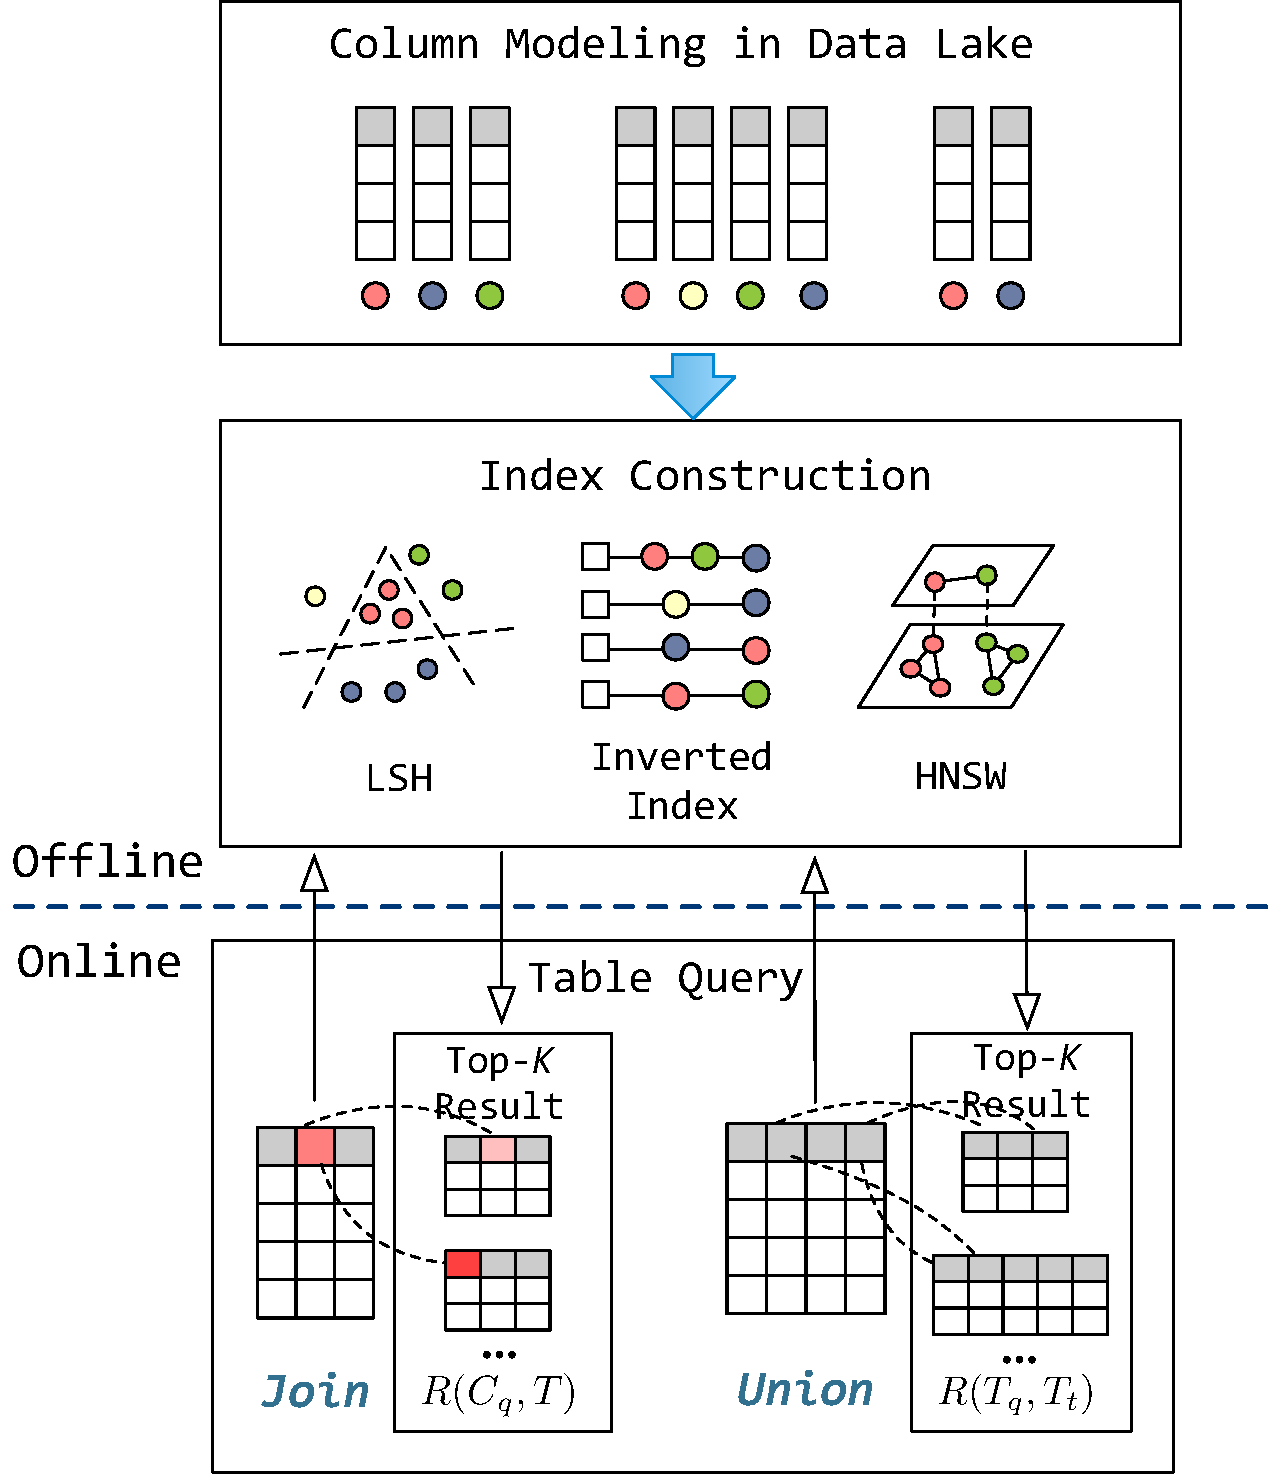
\includegraphics[width=0.95\linewidth]{fig/framework.pdf}
	\caption{Table Discovery in Data Lake.}
	\label{fig:framework}
\end{figure}




%Building upon the column encoders, we leverage cosine similarity between column embeddings to establish the column union ability score. Subsequently, we devise a bipartite matching-based method for calculating the table union ability score. Our approach introduces a filter-and-verification framework, allowing the application of diverse indexing and pruning techniques to minimize the computational load of the resource-intensive bipartite matching.

\iffalse
\subsection{Existing Benchmarks}

{\scriptsize
    
}

Arxiv work~\cite{LakeBench}
Join: 
InfoGather~\cite{InfoGather}, 
Frt12~\cite{Frt12}, 
Lsh Ensemble~\cite{LshEn}, 
Aurum~\cite{Aurum, SemProp}, 
Pexeso~\cite{Pexeso}, 
Josie~\cite{Josie}, 
DeepJoin~\cite{DeepJoin}, 




%ML Join: Metam~\cite{Metam}, Leva~\cite{Leva}, Arda~\cite{Arda}, AutoFeature~\cite{AutoFeature}


Union: 
InfoGather~\cite{InfoGather}, 
Frt12~\cite{Frt12}, 
D3L~\cite{D3L},
TUS~\cite{TUS}, 
Aurum~\cite{Aurum, SemProp}, 
Santos~\cite{Santos}
\fi



%ML Union: Starmie~\cite{Starmie}, AutoData~\cite{AutoData}
%!TEX root = ../main.tex
\section{Benchmark Design} 
In this section, we first introduce the design goals of \sys benchmark for table discovery tasks, and then present how to generate the \sys benchmark consisting of datasets, queries and ground truth.

\subsection{Design Goals}
We design the table discovery benchmark by the 
benchmark design criteria proposed by Jim Gray.

\noindent\textbf{Relevance.}
The benchmark covers a wide range of table discovery characteristics. First, in terms of the data lake, we incorporate 4 lakes with size ranging from 10GB to 1TB, and with column number ranging from \cc{1 million} to 10 million. Second, in terms of the queries, with the help of much human efforts, we create and label more than 10 thousand table queries that cover various query characteristics, including column semantic, column overlapping, column size, etc.



\noindent\textbf{Scalability.} The benchmark involves much larger data lakes than existing data lakes for table discovery. The data lake size should be considered from two aspects. One is the normal total storage size that is highly related  to the average table size  and the number of tables. The other is the number of total columns because almost all table discovery algorithms build index and search over a large number of columns.  \sys involves up to 1 TB data lake and 10 million columns, which is sufficient enough to evaluate the scalability.




\noindent\textbf{Simplicity.} The benchmark designs easy-to-use APIs to support table discovery in data lakes. Users can simply leverage few lines of codes to query our benchmark datasets using different algorithms and compare with them.
\cc{seems limited}





\begin{figure}[h]
	\centering
	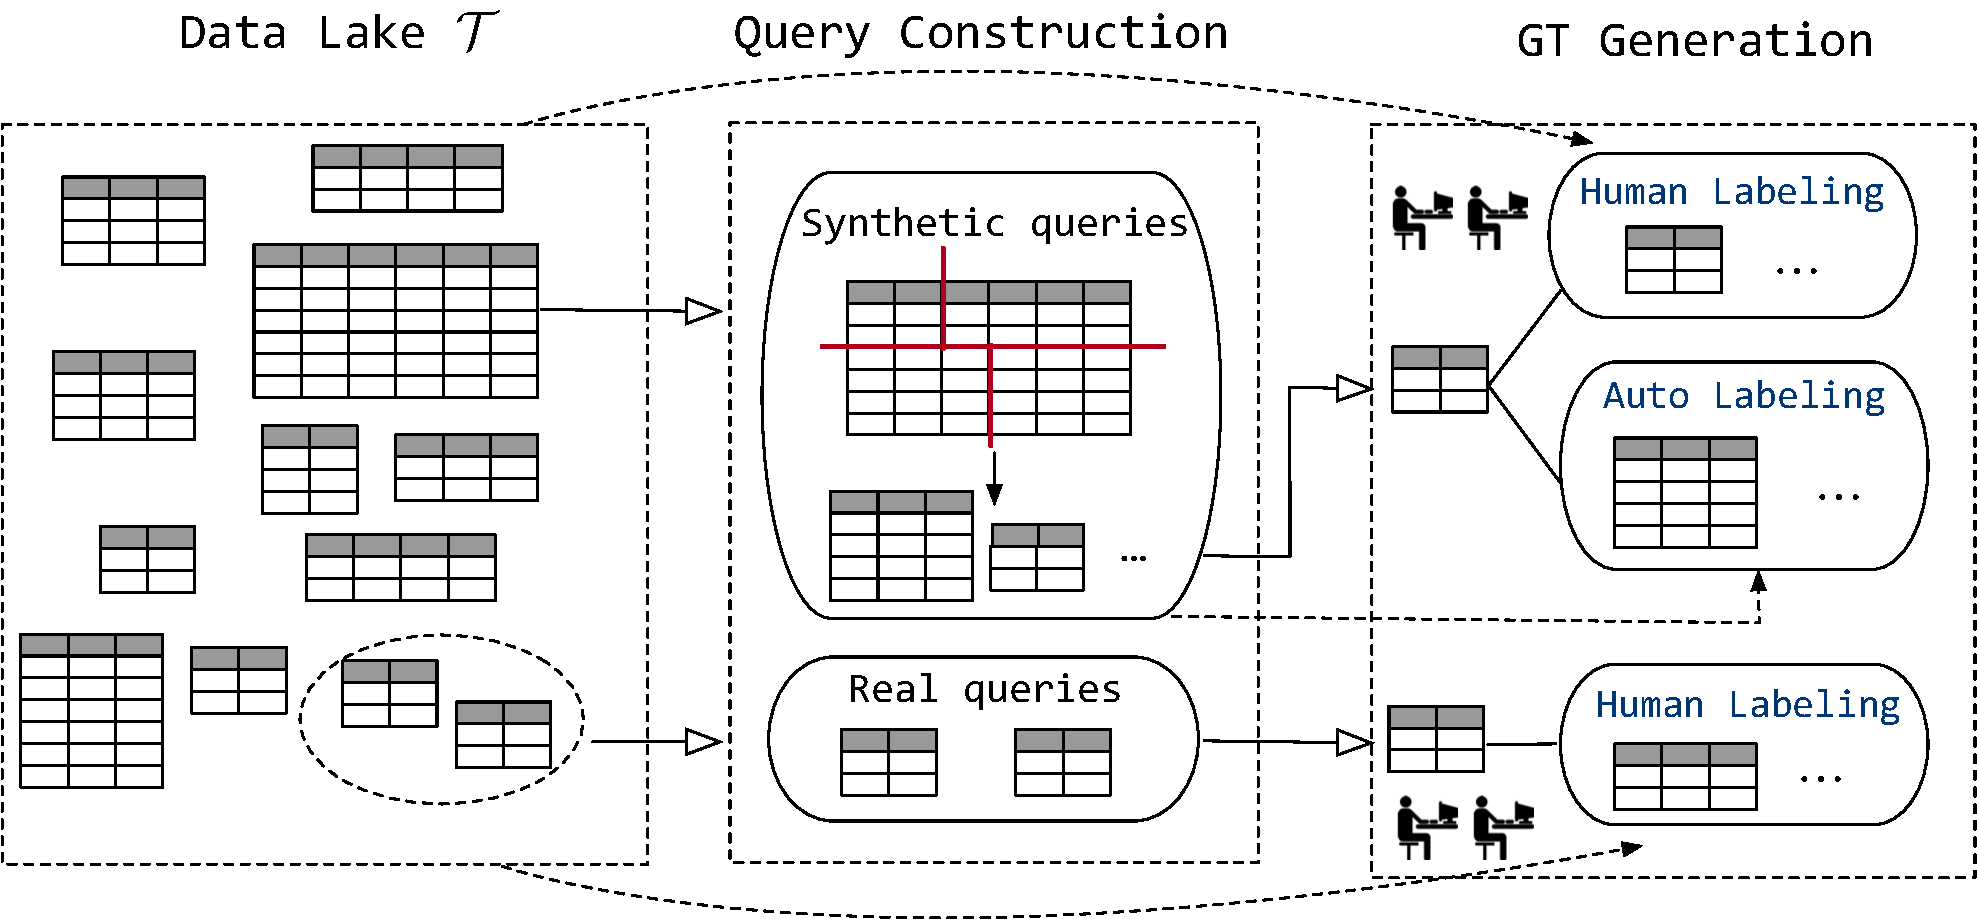
\includegraphics[width=1\linewidth]{fig/benchmark.pdf}
	\caption{Overview of \sys Construction.}
	\label{fig:benchmark}
\end{figure}



\subsection{Benchmark Overview}
In this subsection, we overview the pipeline of our benchmark design. Overall, as shown in Figure~\ref{fig:benchmark}, we first collect the datasets, then construct queries and generate ground truth for these queries. Finally, we implement various table discovery algorithms, analyze their performance from multiple perspectives, and design easy-to-use APIs.

\noindent\textbf{Datasets.}
We build 4 data lakes from OpenData~\cite{OpenData} and WebTable~\cite{WebTable}. For each data source, we create a small and large data lake respectively.

For OpenData~\cite{OpenData}, the original dataset contains XX tables, 

For WebTable~\cite{WebTable}, the original dataset contains XX tables, 


+ Statistics of collected datasets.

+ Clean the datasets.

+ Remove sth.

%Table~\ref{table} summarizes the statistics of collected datasets.


\noindent\textbf{Query Construction.} We use two methods to construct join \& union search queries.

\noindent \underline{\textit{Real queries.}}  A direct way  is to use real tables  as queries, so we  extract  $Q\subset \lake$ as a set of queries. However, in real scenarios, the table search results are likely to be sparse, so in all previous benchmarks, they construct synthetic queries based on big tables, and we conduct this in a similar way as follows.

\noindent \underline{\textit{Synthetic queries.}} The basic idea is to split large tables into multiple small ones. As shown in Figure~\ref{fig:benchmark}, generally, we split from two perspectives, namely row-level and column-level splitting. 
Basically, row-level splitting mainly generates unionable tables, while column-level splitting mostly generates joinable tables.
These small tables are then put into the data lake and they can also serve as queries.
%Split large tables into small ones, which are put into the data lake, and then use some of the small ones as queries.  


\noindent\textbf{Ground Truth Generation.} For different query construction methods, the ways of ground truth (GT) generation are different, as shown in Figure~\ref{fig:benchmark}.

 \noindent \underline{\textit{GT generation for real queries.}} An ideal ground truth generation method is that for each of queries, we ask the humans to label whether all tables in $\lake$ can be join/union with the query, which is prohibitively expensive. A natural solution is to leverage a rough search  method to retrieve a number of candidate tables that have a relatively high relevance with the query table, \ie a high recall, and then ask the humans to manually check these candidates.
 
 \noindent \underline{\textit{GT generation for synthetic queries.}} We can see from  Figure~\ref{fig:benchmark} that the ground truth of synthetic queries consists of two parts. 
 On the one hand, since each synthetic query is obtained by splitting from a big table, there exist multiple tables splitted from the same table that are joinable/unionable with the query. 
  On the other hand, very likely, there  still exist joinable/unionable tables in $\lake$ besides the above  splitted ones.  Therefore, we leverage the above method for  real queries to label more ground truth via humans.




\iffalse
+ Classify: 

\quad\quad -- Column type (string, number, category)
 
\quad\quad -- Fake or real
  
\quad\quad -- Selectivity

\quad\quad -- Size

\noindent\textbf{Ground Truth Creation.}
\fi


\noindent\textbf{Method Evaluation.} 

\cc{How to category}

+ \cc{Join/Union}

+ \cc{Schema matching}

+ Hash-based

+ Inverted index 

+ Pre-trained language model (HNSW)


\noindent\textbf{API Design.}

    \begin{table*}[t]
        \centering
        \caption{Table Discovery Methods.}
        \begin{tabular}{|c|c|c|c|c|cccc|}
            \hline
            \multirow{2}{1cm}{\textbf{Methods}} & \multirow{2}{0.6cm}{\textbf{Task}} & \multirow{2}{0.8cm}{\textbf{Index}} & \multirow{2}{1.6cm}{\textbf{Embedding}} & \multicolumn{2}{c}{\textbf{Offline Process}} & \multicolumn{2}{c|}{\textbf{Online Process}} \\
            &&&&Time Comp.    & Space Comp. & Time Comp. & Space Comp. \\ 
            \hline
            \josie~\cite{Josie} & J & Inv. index & \XSolidBrush  & O$(\cellvaluenum + \rawtokennum \log \rawtokennum)$         & O$(\rawtokennum)$                   & O$(\positinglistlen log \positinglistlen)$         & O$(\positinglistlen)$    \\
            \hline
            \lsh~\cite{LshEn} & J & LSH & \XSolidBrush& O$(\columnnum)$        & O$(\columnnum \times \minhashlen)$                   & O$(\querycolumnnum)$                & O$(\querycolumnnum \times \minhashlen)$  \\
            \hline
            \pex~\cite{Pexeso} & J &  Inv. index& \Checkmark  & O$(\rawtokennum)$        & O$(\rawtokennum)$                   & O$(\querycellvalue + \log \querycellvalue \times \log \rawtokennum)$                & O$(\querycellvalue)$     \\
            \hline
            \deepjoin~\cite{DeepJoin} & J & HNSW & \Checkmark & O$(\columnnum)$         & O$(\columnnum)$                   & O$(\log \columnnum)$                & O$(\columnnum)$  \\
            \hline
             \tus~\cite{TUS} & U & LSH & \Checkmark  & O$(\cellvaluenum + \columnnum)$         & O$(\columnnum \times \minhashlen)$    & O$(\querycolumnnum)$               &  O$(\querycolumnnum \times \minhashlen)$     \\
            \hline
            \dlll~\cite{D3L} & U & LSH & \Checkmark& O$(\cellvaluenum + \columnnum)$          & O$(\columnnum)$                   & O$(\querycolumnnum \times \dlllneighbornnum)$                & O($\querycolumnnum$)      \\
            \hline
            \starmie~\cite{Starmie} & U & HNSW & \Checkmark & O$(\columnnum)$         & O$(\columnnum)$                   & O$(\log \columnnum)$                & O$(\columnnum)$   \\
            \hline
            \santos~\cite{Santos} & U & Inv. index & \XSolidBrush & O$(\rawtokennum)$         & O$(\rawtokennum \times \columnnum {\averagetargetcolumnnum}^2)$    & O$(\querycellvalue + \santosneighbornnum)$               & O$(\querycellvalue)$  \\
            \hline
            \frt~\cite{Frt12} & J \& U & \XSolidBrush & \XSolidBrush &  O$(\columnnum)$        & O$(\columnnum)$    & O$( \tablenum \times {(\querycolumnnum + \averagetargettuplenum)}^3)$               & O$({\averagetargettuplenum}^2)$    \\
            \hline
            \infogather~\cite{InfoGather} & J \& U & Inv. index & \XSolidBrush & O$(\columnnum^2)$   & O$(\columnnum^2)$    & O$(\querycolumnnum \times \inforneighbornnum \log \inforneighbornnum)$              & O$(\inforneighbornnum )$   \\
            \hline
            \aurum~\cite{Aurum} & J \& U & LSH & \Checkmark  & O$(\columnnum)$         & O$(\columnnum)$                   & O$(\log \columnnum)$                & O$(\columnnum)$   \\
            \hline
            Pretrain-based Method~\cite{} & U & HNSW & \Checkmark   & O$(\columnnum)$         & O$(\columnnum)$                   & O$(\log \columnnum)$                & O$(\columnnum)$ \\
            \hline
        \end{tabular}
        \label{table:methods}
        
    \end{table*}

\begin{table*}[!ht]
	\centering
	\caption{The Meaning of Different Symbols.}
	\begin{tabular}{cc}
		\hline
		Symbol & Meaning \\ \hline
		$\mathcal{B}$ & Number of columns in the query table $\qtable$  \\
		$\mathcal{N}$ &The total number of columns in all tables in the data lake $\lake$ \\
		$\mathcal{K}$ & The number of non-distinct cell values in all tables in the data lake $\lake$   \\
		$\mathcal{R}$ &The number of distinct cell values in all tables in the data lake $\lake$ \\
		$\mid \mathcal{T} \mid$ & Number of tables in the data lake $\lake$  \\
		$\mathcal{X}$ &The total number of tuples in all tables in the data lake $\lake$ \\
		$\mathcal{A}$ & The number of non-distinct cell values in query table $\qtable$  \\
		
		$\mathcal{L}$ & The length of positing list in \josie  \\
		$\mathcal{H}$ & The dimension of minhash vector \\
		$\mathcal{P}$ & The number of partition in \lsh\\
		$\mathcal{D}$ & The number of neighbors in \dlll\\
		$\mathcal{I}$ & The number of neighbors in \infogather\\
		$\overline{\mathcal{O}}$ & The average number of tuples in target column\\
		%


%fake方法造query:就是先选一个行和列都比较多的大表,然后随机选择num列(num为随机数),并且打乱这些列的顺序,再添加了一列随机数;竖着切成几个小表之后,再随机选择num行(num为随机数),并且打乱这些行的顺序,同时,选择横着切表之前的1/4行作为切完之后各个小表之间的overlap。

%不fake方法造query:随机抽选一些候选表出来,然后再人工抽取一些人能识别出来表格主题的表(方便后续ground truth的标注)

%fake方法定ground truth: 首先,竖着切之后,判断各个小表有没有属性重复,有的话,两个表之间视为可以join。除此之外,横着切生成的不同小表,由于它们之间一定会有overlap和属性重复,所以两两之间视为可union

%不fake方法定ground truth:根据不fake的方法造出来的query,利用一些简单的相似性判断捞出一些候选表,再进行人工标注

	
	\end{tabular}
	\label{symbol_table}
\end{table*}




%!TEX root = ../main.tex
\section{Datasets}


%!TEX root = ../main.tex
\section{Query \& ground truth Construction}

\subsection{Synthetic query generation}
In this part, we will discuss how to split large tables and generate the corresponding ground truth.

\noindent \textbf{Choosing Large Tables.} 
To split a base table into multiple small synthetic queries, it is usually necessary to use a large base table with more rows and columns. To achieve this, we sorted all the lake tables by multiplying the number of rows and columns of each table. Tables with rows and columns greater than a certain threshold were selected, and in order to ensure the diversity of synthetic queries, we manually selected tables with differenet semantics as the base tables.

\noindent \textbf{Synthetic Query Construction.} 
To generate syhthetic queries that are relatively realistic, including randomness and a certain level of difficulty. We mainly use two methods to generate synthetic queries for join and union case, which involve horizontal and vertical table splitting.

\noindent \underline{\textit{Union Case.}}  To generate synthetic queries for the unionable case, it is essential for two small tables to share identical columns. Consequently, we generate unionable scenarios by partitioning the original base table both horizontally and vertically, ensuring there is no overlap in rows and varying the extent of column overlap. First, we horizontally split the table into several parts, then randomly select several columns from each part as column overlap. After that, we select the remaining columns that are not duplicate as supplementary columns for each small table, and thus forming the synthetic queries for the union case.

\noindent \underline{\textit{Join Case.}}  Joinable tables must share at least one common joining column, and unlike unionable tables, they should exhibit a substantial row overlap. To construct this case, similar to the method used in the union case we first vertically split the base table into several tables while retaining varying proportions of overlapping columns (e.g., 1 column, 30\% of columns, 50\%, etc.). Furthermore, we horizontally divide the split tables with varying row overlap percentages (in our case,20\%, 35\%, 50\%, etc.). 

\noindent \textbf{Ground Truth Generation.} 
During the process of constructing synthetic queries, ground truth are also generated accordingly.
\noindent \underline{\textit{Union Case.}}  
As mentioned above, we first divide the base table horizontally into different parts, and then select some small tables with common columns in each part. As a consequence, these small tables are unionable in pairs, so we mark them as ground truth.
\noindent \underline{\textit{Join Case.}} 
Similarly, when constructing the syhthetic quries for join case, we initially vertically partition the base table into multiple tables, preserving different percentages of overlapping columns (varying from 1 column to 50\% of columns). These overlapping columns and partition tables correspond to the query table and ground truth of the join case respectively.
%+ How to choose large tables.

%+ How to split.

%+ How to generate the ground truth.
\subsection{Basic search for candidate generation}
In this part, for each synthetic or real query, we design a basic search algorithm to retrieve  candidate joinable/unionable tables from the data lake. 

\noindent \underline{\textit{Union Case.}}  
To retrieve the unionable tables from the data lake, it not only requires considering $(\romannumeral1 ).$  the semantics of the corresponding columns in two tables (i.e. only considering the semantics between individual column pairs), but also $(\romannumeral2 ).$ the semantics between two tables (i.e. the relationships and semantics between different columns in the same table),  Therefore, we used multiple methods that consider these two semantics separately to obtain results on the query table. Specifically, we use \starmie,\santos and SATO. After that, we take the union of these results as the candidate tables and label them by experts.

\noindent \underline{\textit{Join Case.}}  
In the case of joining tables, several considerations are essential:$(\romannumeral1).$ the semantics of corresponding columns in both tables. $(\romannumeral2).$ analyzing the relationship between the two tables, $(\romannumeral3).$ ensuring there is an overlap in cell values between the corresponding columns. Consequently, We used method that considers both $\romannumeral1$ and $\romannumeral2$, namely \deepjoin, and method that considers $\romannumeral3$, namely \josie, to obtain candidate tables respectively.

\noindent  \underline{\textit{Number of Candidate Tables.}}  The number of candidate tables we obtained was determined by experts. We first set an accuracy threshold (i.e. 70\%), and then manually judged that when the number of candidate tables reached a certain number, their corresponding accuracy was lower than the threshold we set. At this point, the number of selected tables is the final number of our candidate tables.
%+ How to guarantee high recall

%+ Details

\subsection{Human labeling}
In this part, we ask the human experts to label the candidates for each query. In order to improve the efficiency of experts data labeling, we built a webpage for labeling the ground truth of both join and union case.

%+ Example shown to the experts.

\noindent \textbf{Labeling Interface.} 
The labeling interface we built is shown in the Figure ~\ref{fig:interface}, we demonstrate the interface for union case and the interface for join case is similar. The interface is mainly divided into three parts in a vertical direction. We will further explain how each part works.

\noindent \underline{\textit{Query Table Specification.}}  
As shown in Figure ~\ref{fig:interface}-\raisebox{.3pt}{\textcircled{\hspace{-0.08cm} \raisebox{-.5pt}{1}}}, this section displays a list of query tables to be labeled.  The figure shows a list of ten query tables and the user can select a specific query table, whose information will be dispalyed in Figure ~\ref{fig:interface}-\raisebox{.3pt}{\textcircled{\hspace{-0.08cm} \raisebox{-.5pt}{2}}}.

\noindent \underline{\textit{Metadata of Query Table.}}  When selecting the corresponding query table,  its corresponding information is to be visualized.(see Figure ~\ref{fig:interface}-\raisebox{.3pt}{\textcircled{\hspace{-0.08cm} \raisebox{-.5pt}{2}}}). For example, after the user chooses the first query table, its main information, including the metadata and the table itself  will be shown. We can see that for the query table \cc{XX}, its column names varying from \cc{XX} to \cc{XX}. Furthermore, for column \cc{XX}, it mainly consists of two distinct cell values, namely \cc{XX} and \cc{XX}. These meta information are displayed above the query table as auxiliary information to help users better determine whether two tables can be joined or unioned.

\noindent \underline{\textit{Candidate Table Specification.}} The functions of this part are similar to that of Query Table Specification (see Figure ~\ref{fig:interface}-\raisebox{.3pt}{\textcircled{\hspace{-0.08cm} \raisebox{-.5pt}{3}}}). In this part, users can select a candidate table and get some relevant visualizations they want. For example, when choosing candidate table \cc{XX}, the interface will show its column name and the corresponding range of cell values for each column.

\noindent \underline{\textit{Metadata of Candidate Table.}}  Similarly, this part provides the explanations in plain text for the metadata of a specific candidate table, which will help the users to better understand the meaning of the entire table.  The users can click the “more” button for more visualization details (see Figure ~\ref{fig:interface}-\raisebox{.3pt}{\textcircled{\hspace{-0.08cm} \raisebox{-.5pt}{4}}}).

\noindent \underline{\textit{Labeling Area.}} The users may select a specific query table and its unionable candidate table and further conduct a labeling operation in the labeling area of the interface (see Figure ~\ref{fig:interface}-\raisebox{.3pt}{\textcircled{\hspace{-0.08cm} \raisebox{-.5pt}{5}}}). Suppose that the user chooses the query table \cc{XX} and candidate table \cc{XX}, by clicking the "union" button, the interface will initiate a process to gather labeled data and store it in the backend database. Upon successful labeling, the system will prompt the user for confirmation.


\begin{figure*}[h]
	\centering
	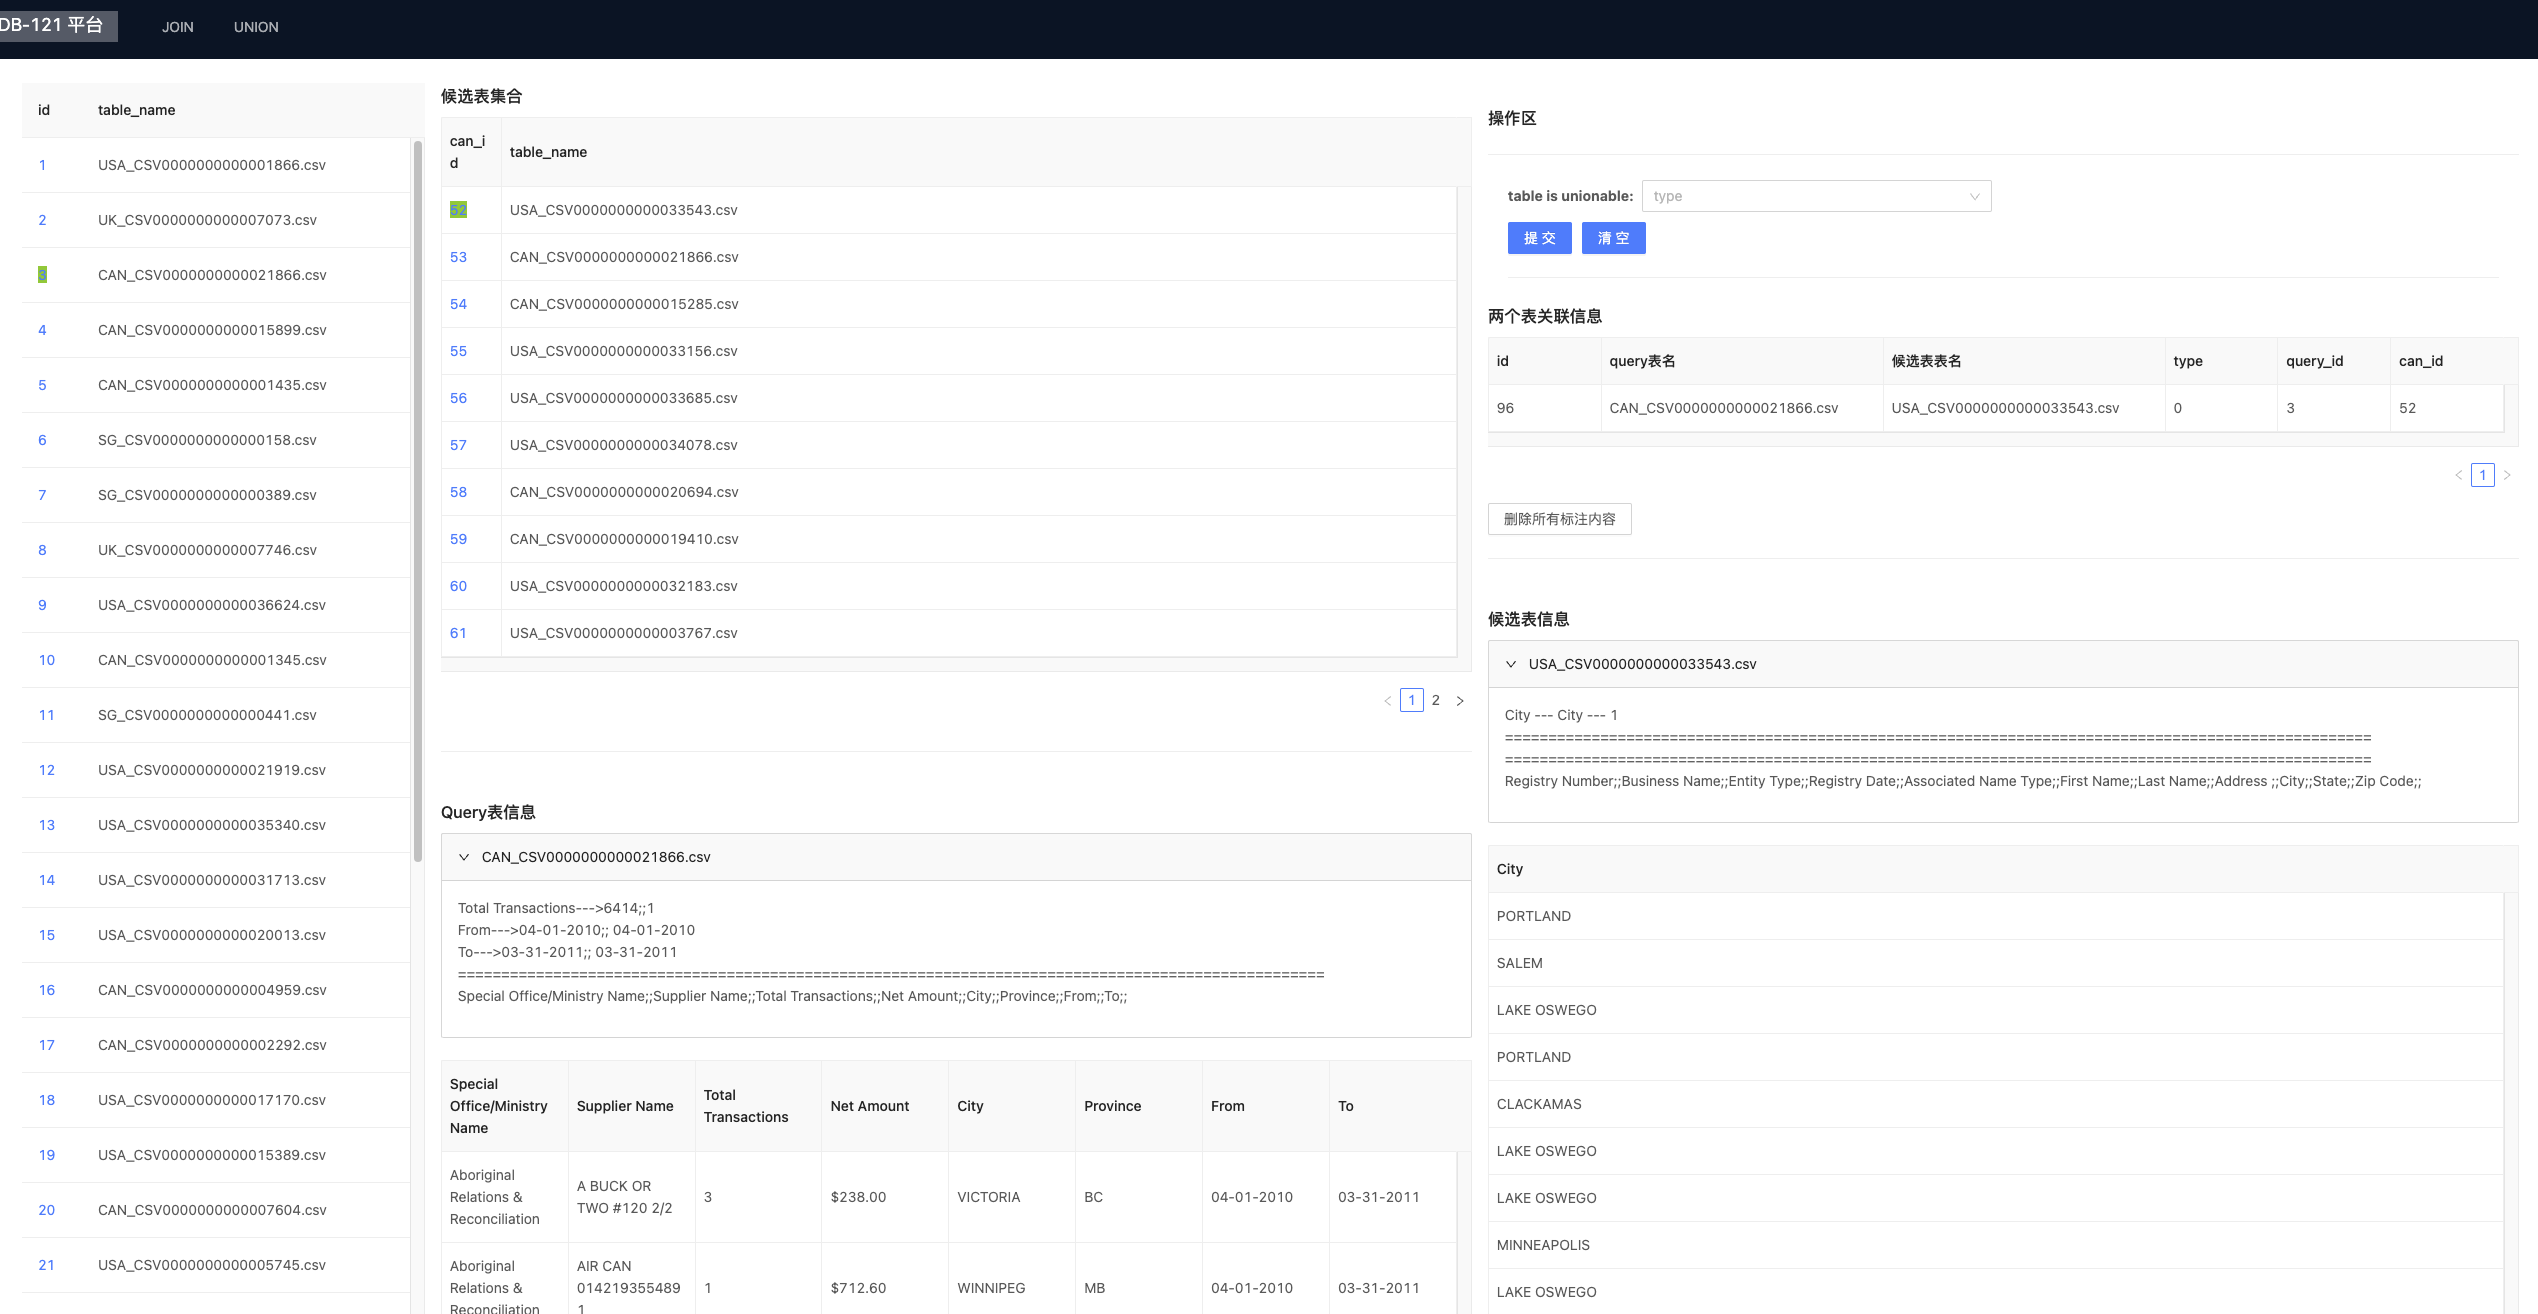
\includegraphics[width=1.0\linewidth]{fig/interface.png}
	\caption{Labeling Interface of Webpage.}
	\label{fig:interface}
\end{figure*}

\noindent \textbf{Labeling Statistics.} 
We have count some statistical information during manual labeling, as show in Table ~\ref{Table:humanLabeling}. For OpenData Large, this dataset has a total of  \cc{XX} query tables to be labeled, with an average of 20 candidate tables matching each query table. Therefore, we have 10 experts and spent a total of approximately \cc{XX} hours completing the labeling work. Similarly, for WebTable Large, we also have 10 experts and spent a total of approximately \cc{XX} hours for labeling. This is because this dataset has \cc{XX} query tables in all that need to be labeled, and each table has an average of 20 corresponding candidate tables.

\begin{table}[t]
	\centering
	\caption{Statistics of Human Labeling.}
	\begin{tabular}{|c|c|c|c|c|c|}
		\hline
		\centering
		Data Lake  & \#-Query Tables & $\#$-People & Time.   \\
		\hline  
		OpenData Small& 914  & 10 & 10h   \\
		\hline
		OpenData Large& 1,448  & 10  &  17.5h   \\
		\hline
		WebTable Small& 1,745   & 10 &  20h  \\
		\hline
		WebTable Large& 2,245  & 10 &  30h  \\
		\hline
	\end{tabular}
	\label{Table:humanLabeling}
	
\end{table}
%!TEX root = ../main.tex
\section{Approach Evaluation} 
In this section, we  evaluate existing table discovery approaches in \sys benchmark, and analyze the results.
We would like to answer the following questions. 
(1) What are the concrete solutions of different methods to solve the table discovery problem?
(2) How is the scalability of different algorithms, especially on large-scale datasets. 
(3) Given all queries, what are the precision and recall of different algorithms on the benchmark datasets on average?
(4) Given queries with different characteristics, then how about the precision and recall?

\subsection{Existing Methods}




\subsubsection{Table Discovery Approaches}
We naturally categorize existing approaches into three categories, namely approaches for join, union, and both of them.
Table~\ref{table:methods} shows the details of different methods. 

\noindent\textbf{Table Join Search.}
 (1) \josie aims to find joinable tables in data lake via set similarity search. Based on the intuition that two joinable columns have many overlap values, given the query table $\qtable$ and query column $\qcolumn$,  \josie considers $\qcolumn$ as a set, and finds the  exact top-$k$ columns in the data lake that have high overlap set similarities with $\qcolumn$. To be specific, overlap set similarity refers to the intersection value between two columns. To achieve this efficiently, \josie builds the inverted index that maps    distinct cell values and sets (columns) that contain each corresponding value. Then given a query column, the inverted index can help to identify candidate columns with overlap values in the data lake, a cost model is introduced to quickly eliminate unqualified candidates. 

 \noindent  (2) Similar to \josie, \lsh also considers the set overlap between columns to determine whether two tables can be joined.  Different from \josie that computes the exact top-$k$ columns, it estimates the proportion of overlap values (\ie Jaccard similarity) using an index structure based on MinHash LSH and return the columns with the proportions larger than a threshold, which is  built by two stages. First, all columns in the data lake is partitioned disjointly based on their cardinalities. Second, a MinHash LSH index for each partition is constructed and dynamically tuned considering its customized Jaccard similarity threshold. The key contribution is a cost model to conduct an optimal data partitioning for the LSH index, such that the false positive rate could be minimized if an ideal Jaccard similarity filter is used in each partition.
 
 %is enable to obtain high accuracy over a large and skewed domain distributions. 

 

 \noindent  (3) \pex considers the semantics of textual columns to capture the column similarity, unlike the above two methods that just consider exact match among cell values of columns. To be specific, it first encodes column values in the data lake into high-dimensional vectors using fastText~\cite{}, which are then indexed by an inverted index and a hierarchical grid. When a query $\qcolumn$ comes, a block-and-verify strategy is applied to efficiently compute the cosine similarity between vectors.
 
 
 
 \noindent  (4) \deepjoin also considers the column semantics represented by vectors. Different from \pex that directly encodes columns into vectors,  \deepjoin involves a training process fine-tuning based on DistilBERT~\cite{} and MPNet~\cite{}. This process feeds a pair of columns into the pre-trained language model,  outputs two vectors and computes their cosine similarity, which is used to compute the loss by comparing with the similarity between this pair of columns. Afterwards,  columns in the data lake are transformed into vectors that are indexed using HNSW~\cite{}. When a query $\qcolumn$ comes, it is also transformed into a vector and similar columns that are likely to be joined with it are retrieved though the HNSW index.
 
 
 


 %deepjoin sufficienctly discuss the above methods.

\noindent\textbf{Table Union Search.}
 (1) \tus first defines the table union search problem that discovers tables from the data lake that can union with the query table. If two tables have multiple columns (\ie attributes) with similar domains, they are likely to be unioned. To determine the unionable attributes, three statistical models that respectively consider value overlap , ontology similarity and natural language similarity are incorporated. Then, given any pair of columns,  \tus leverages a data-driven  method to judiciously choose the best model to describe their unionbility. Also, a TUS benchmark is proposed to validate the algorithm.  

 \noindent  (2) \dlll also considers the similarity between columns, which are then utilized to union two tables. It considers the column similarity from 5 aspects, namely attribute name, attribute extent, word-embedding of attributes, format representation and domain distribution. Then \dlll leverages a weighting strategy that computes a more accurate similarity for columns.
 
  \noindent  (3) \santos. The above methods mainly consider  the semantic similarity of  schemes and cell values of columns to determine whether two tables can be joined.
   \santos further improves the accuracy by incorporating the semantic relationships between pairs of columns. To be specific,  it can leverage a KB to annotate a semantic graph for columns within a table. When a query table comes, the graph will be compared with graphs in the data lake such that the column semantics can be well considered. In most scenarios, it is hard for a KB to well cover the values in a real data lake, so \santos proposes a synthesized KB to annotate the column relationships using the knowledge in the data lake.

 \noindent  (4) \starmie focuses on union tables based on large  pre-trained language models. To be specific, a lightweight contrastive learning method is applied to train 
column encoders in an unsupervised way, which captures rich information of contextual semantics. Then, columns in data lake are represented as vectors and the HNSW index is applied to accelerate the query efficiency.


\noindent\textbf{Methods can be used for Join \& Union.}
  (1) \infogather aims at augmenting entities or attributes from a large corpus of HTML tables for a given table, which can be regarded as table union or join search. The basic idea is to first achieve a holistic matching across all tables, and then  given a query table,  \infogather finds tables that can be unioned or joined using direct or indirect matching among tables in the data lake.
 
 
  \noindent  (2) \aurum can also be utilized to solve  both the table join/union search problems. First, the schema of each column is encoded using word embeddings. Then, all columns are organized as a graph that each node corresponds to a column and each edge connects two nodes with similar embeddings. When a query table comes, all columns in the table will also be encoded and hashed to find similar columns in the data lake, and  the nearby tables are also retrieved based on the graph. Finally, the join/union scores are computed based on those candidate tables.  
  
    \noindent  (3) \frt introduces a framework that captures different relatedness of tables, which are then utilized for union or join. For union,  \frt considers entity consistency, entity expansion and schema consistency to align two tables. For join, \frt considers the coverage of entity sets of two columns.

\subsection{Evaluation}

\noindent\underline{Metric}

\noindent\underline{Effectiveness}

\noindent\underline{Efficiency}

\noindent\underline{Threshold}

\noindent\underline{Buckets!!!}





%!TEX root = ../main.tex
\section{API Design}
%!TEX root = ../main.tex
\section{Related Work}

\normalem
\bibliographystyle{ACM-Reference-Format}
\bibliography{ref}

\end{document}
\endinput
